\chapter{提案手法}
\label{proposed}
\section{提案}
\begin{itemize}
  \item ポーズ推定ライブラリであるMediaPipePose\cite{mediapipe_pose_landmarker}を用いて各関節の座標を取得する。その座標から関節角度を計測し、理想形との差異を測定する。
  \item 音声で大まかなフィードバックを与えることで利用者本人の内在的フィードバックによるポーズ習得をさせる。
\end{itemize}
関節の座標同士を繋げ、ボーンを推測し、隣り合うボーンの角度を計測する。その角度をそれぞれの関節でシステムに登録した理想の角度と比較し、差異を計測する。
それぞれの関節において理想の角度との差を計算し、その差が一番大きい関節に対して音声でフィードバックを与える。

\section{実装}
実装は図\ref{fig:system_figure}のように行った。
\begin{enumerate}
  \item webカメラでポーズを撮影
  \item MediaPipePoseを用いて各関節の座標を推測
  \item フィードバックとして読み上げる言葉をVOICEVOXに送信
  \item VOICRVOXで音声データを生成
  \item PCのスピーカーでユーザーへフィードバック
  \end{enumerate}

\begin{figure}[htbp]
  \begin{center}
      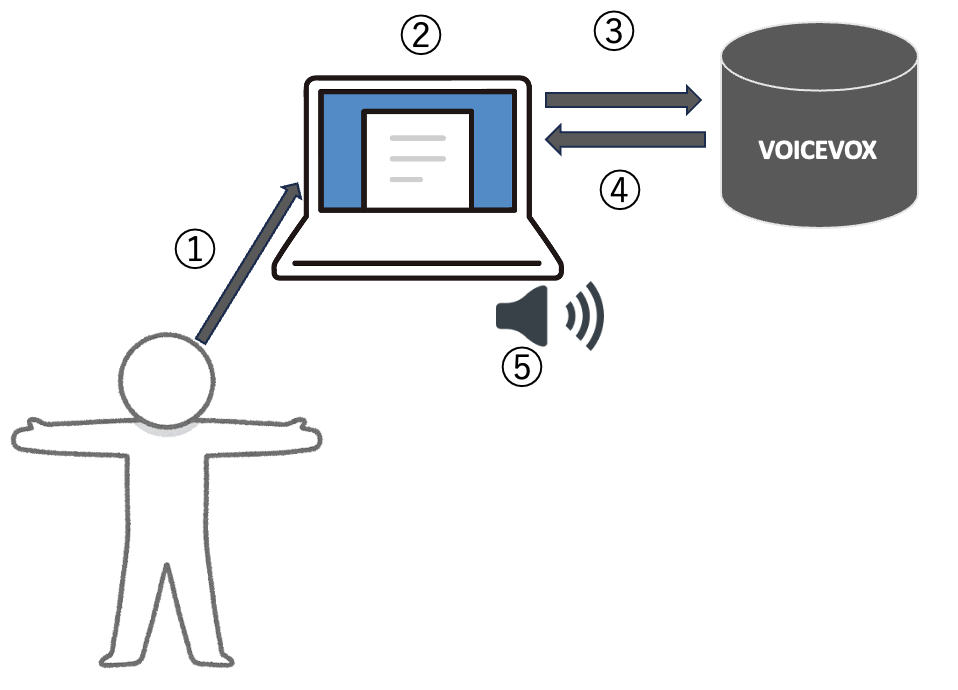
\includegraphics[width=7cm]{figures/system_figure.png}
      \caption{構成図}
      \label{fig:system_figure}
  \end{center}
\end{figure}

